\section{Three-flavor \chpt\ to leading order}
\label{section: three-flavor chpt to leading order}



\subsection{Ground state}

For $N_f = 3$, the generators are $T_\alpha = \frac{1}{2} \lambda_\alpha$, where $\lambda_\alpha$ are the Gell-Mann matrices, as shown in \autoref{section: algebra bases}.
The mass matrix is now
%
\begin{equation}
    m = 
    \begin{pmatrix}
        m_u & 0 & 0 \\
        0 & m_d & 0 \\
        0 & 0 & m_s
    \end{pmatrix},
\end{equation}
%
and the charge matrix is
%
\begin{equation}
    Q = \frac{1}{3}
    \begin{pmatrix}
        2 & 0 & 0\\
        0 & -1 & 0\\
        0 & 0 & -1
    \end{pmatrix}
    = \frac{1}{2} \left( \lambda_3 + \frac{1}{\sqrt{3}} \lambda_8 \right).
\end{equation}
%
The leading order Lagrangian still has the same form,
%
\begin{equation}
    \label{leading order three-flavor lagrangian}
    \Ell_2 
    = \frac{1}{4}f^2 \Tr{\nabla_\mu \Sigma \nabla^\mu \Sigma^\dagger}
    + \frac{1}{4}f^2 \Tr{\chi \Sigma^\dagger + \Sigma \chi^\dagger}
    + e^2 C \Tr{\Sigma Q \Sigma^\dagger Q},
\end{equation}
%
where
%
\begin{equation}
    \chi = 2B_0 m =  \frac{2}{3} M_1^2 \one + M_2^2 \lambda_3 + M_3^2 \lambda_8,
\end{equation}
%
and
%
\begin{equation}
    M_1^2 = B_0 (m_u + m_d + m_s), \quad
    M_2^2 = B_0 (m_u - m_d), \quad
    M_3^2 = \frac{1}{\sqrt 3} B_0 (m_u + m_d - 2m_S).
\end{equation}
%
To find the ground state, we start with $e = 0$.
The covariant derivative is then
%
\begin{equation}
    \nabla_\mu \Sigma = \partial_\mu \Sigma - i [v_\mu, \Sigma], \quad 
    v_\mu = \mu \delta^0_\mu,
\end{equation}
%
Here, $\mu$ is the chemical potential matrix,
%
\begin{equation}
    \mu = 
    \begin{pmatrix}
        \mu_u & 0 & 0 \\
        0 & \mu_d & 0 \\
        0 & 0 & \mu_s
    \end{pmatrix}
    = 
    \begin{pmatrix}
        \frac{1}{3}\mu_B + \frac{1}{2}\mu_I & 0 & 0 \\
        0 & \frac{1}{3}\mu_B - \frac{1}{2}\mu_I & 0 \\
        0 & 0 & \frac{1}{3}\mu_B - \frac{1}{2}\mu_S
    \end{pmatrix}
    = \frac{1}{3}(\mu_B - \mu_S) \one 
    + \frac{1}{2} \mu_I \lambda_3
    + \frac{1}{\sqrt{3}}\mu_S\lambda_8,
\end{equation}
%
where $\mu_B = \frac{3}{2}(\mu_u + \mu_d)$, $\mu_I = \mu_u - \mu_d $ and $\mu_S = \frac{1}{2}(\mu_u + \mu_d)-\mu_s$.
Here, $\mu_u$, $\mu_d$, and $\mu_s$ are the up, down, and strange quark chemical potentials, while $\mu_B$, $\mu_I$, and $\mu_S$ are the baryon, isospin, and strangeness chemical potentials.
The baryon number of all mesons, the $\pi_a$'s, is zero, and $\Sigma$ transforms as $\Sigma \rightarrow \Sigma$ under $U(1)_V$, the corresponding symmetry group.
As a consequence, any result will be independent of $\mu_B$.
We can also see this from the fact that $\mu_B$ only appears with the identity matrix $\one$ in $\mu$.
As a consequence, any dependence on $\mu_B$ in $\nabla_\mu \Sigma$ will vanish as $\one$ commutes with everything.
We will assume $\mu_I, \mu_S>0$.


\subsection{Parametrization}

From the structure constants of $\lie{su}{3}$, \autoref{structure constants su(3)}, we see that we can create three independent $\lie{su}{2}$ sub-algebras.
We introduce the matrices
%
\begin{equation}
    \lambda_Q = \lambda_3 + \frac{1}{\sqrt{3}}\lambda_8, \quad
    \lambda_K = \lambda_3 - \frac{1}{\sqrt{3}}\lambda_8,
\end{equation}
%
which commute, i.e., $[\lambda_Q, \lambda_K] = 0$.
With this, we get the commutation relations
%
\begin{equation}
    [\lambda_i, \lambda_j] = 2i \epsilon_{ijk} \lambda_k,\quad
    ijk \in
    \begin{cases}
        &\{1, 2, 3\}\\ &\{4, 5, Q\}\\ &\{6, 7, K\}.
    \end{cases}
\end{equation}
%
We here define the Levi-Civita symbol by $\epsilon_{123} = \epsilon_{34Q} =\epsilon_{76K} = 1$.
To find the ground state, we define
%
\begin{equation}
    \Sigma_\alpha 
    = \exp{i \alpha n_a \lambda_a} = \cos \alpha + i n_a \lambda_a \sin \alpha,
    \quad \alpha = \frac{1}{f} \sqrt{\pi_a^0 \pi_a^0}, \quad n_a = \frac{\pi_a^0}{\sqrt{\pi_b^0 \pi_b^0}}. 
\end{equation}
%
For $\mu_S = 0$, we expect to recover the results from the two-flavor case, which corresponds to $n_1^2 + n_2^2 =1$, $n_a = 0$ for $i>2$.
As argued earlier, we may choose $n_1 = 0$ without loss of generality, in which case the ground state becomes
%
\begin{equation}
    \Sigma_\alpha^{\pipm} = \exp{i \alpha \lambda_2} = (\one - \lambda^2_2) + \lambda_2^2 \cos\alpha + i \lambda_2\sin\alpha.
\end{equation}
%
If we define $\mu_\Kpm = \frac{1}{2}(\frac{1}{2}\mu_I + \mu_S)$ and $\mu_\Ko = \frac{1}{2}(\frac{1}{2}\mu_I - \mu_S)$, then we can write the external currents corresponding to $\mu_I$ and $\mu_S$ as
%
\begin{equation}
    \mu = \frac{1}{2}\mu_I Q_I + \mu_S Q_8 = \mu_\Kpm Q_{\Kpm} + \mu_\Ko Q_\Ko.
\end{equation}
%
We assume $\mu_I,\mu_S>0$, so $\mu_\Kpm > \mu_\Ko$.
Analogously to how turning up $\mu_I$ leads to a condensate in the first $\lie{su}{2}$ subalgebra, we can expect these chemical potentials to lead to a condensation in their respective subalgebra.
As we work with $\mu_I, \mu_S >0$, we can assume $\mu_\Ko$, in which case we would expect the form
%
\begin{align}
    \Sigma_\alpha^{\Kpm} = \exp{i \alpha \lambda_5} = (\one - \lambda^2_5) + \lambda_5^2 \cos\alpha + i \lambda_5\sin\alpha.
\end{align}
%
Similarly, for $\mu_S<0$, we could set $\mu_\Kpm = 0$ and expect a ground state of the form $e^{i\alpha\lambda_7}$.
In \autocite{kogutQCDSmallNonzero2001}, \citeauthor{kogutQCDSmallNonzero2001} show that exactly this happens. 
At $\mu_\Kpm^2 = m_K^2 = \frac{1}{2}B(m_u + m_d + 2 m_s)$, we get a charged pion condensate, and a neutral kaon condensate at $\mu_\Ko^2 > m_K^2$.
However, these domains are overlapping, so there is a first-order phase transition between the different condensates.
\autoref{fig: phase diagram} show the phase diagram in the $\mu_I, \mu_S$-plane.

\begin{figure}
    \centering
    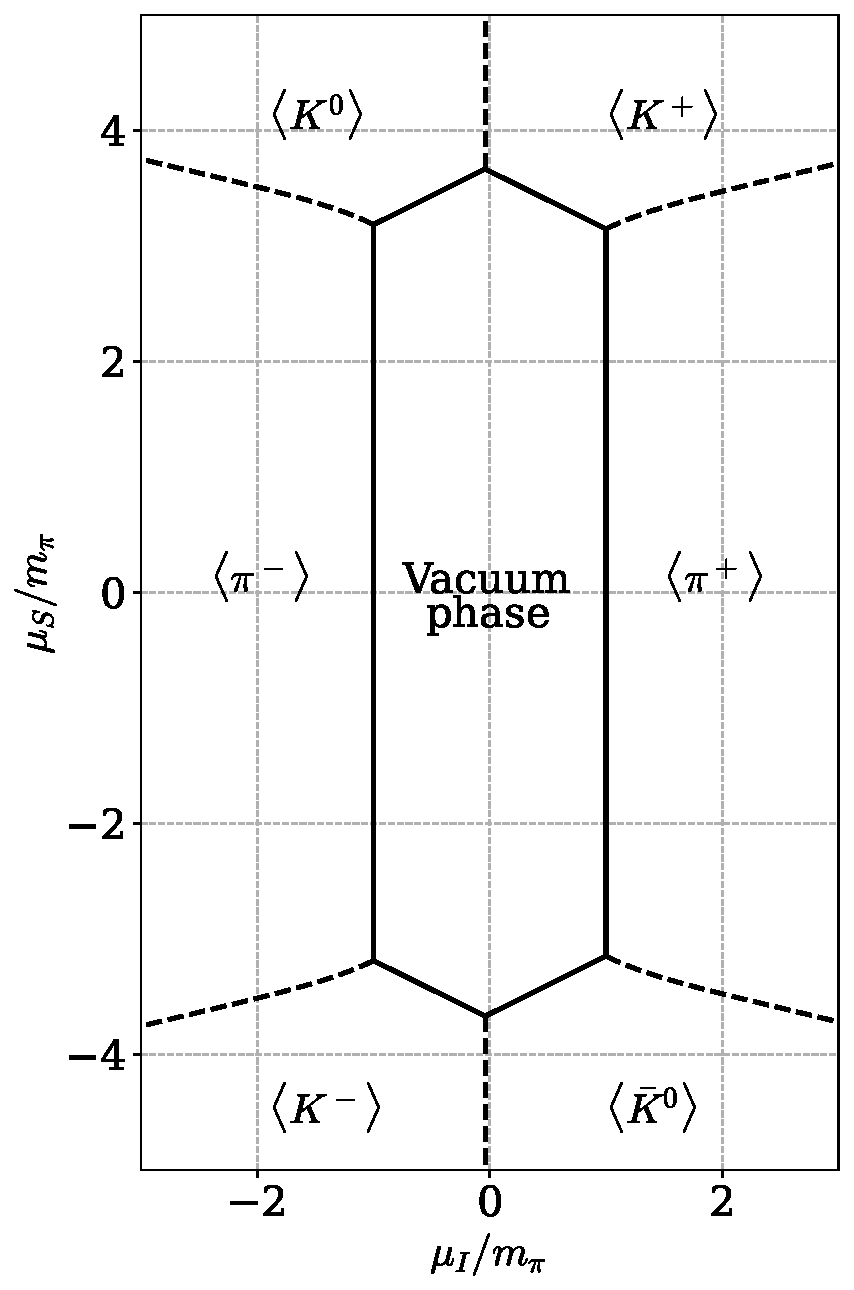
\includegraphics[width=0.6\textwidth]{../scripts/figurer/phase_diagram.pdf}
    \label{fig: phase diagram}
    \caption{Kladd}
\end{figure}



\subsection{Leading order Lagrangian}

Excitations in these ground states are parametrized as
%
\begin{equation}
    \Sigma(x) = A^i_\alpha U(x) \Sigma_0 U(x) A^i_\alpha, \quad
    U(x) = \exp{i \frac{\pi_a \lambda_a}{2 f}}, \quad
    A_\alpha^i = \exp{i \frac{\alpha \lambda_i}{2}},
\end{equation}
%
where $i = 2, 5, 7$ depending on which ground state we are in.
We start working in the pion condensate phase, so $i = 2$, and assume $\mu_I > 0$ and $e = 0$.
Inserting this into \autoref{leading order three-flavor lagrangian}, and expending up to and including $\Oh\left((\pi/f)^2\right)$, we get
%
\begin{align}
    \Ell_2^{(0)} 
    &=
    \frac{1}{2} f^2
    \left(
        \mu_I^2 \sin^2\alpha
        + 2\bar m \cos\alpha
        + m_S
    \right), \\
    \Ell_2^{(1)}
    &=
    -f \mu_I \partial_0 \pi_1 \sin\alpha
    + f \sin\alpha
    \left(
        \mu_I^2\cos\alpha - \bar m^2
    \right)\pi_2, \\
    \Ell_2^{(2)} 
    &= 
    \frac{1}{2}\partial_\mu \pi_a \partial^\mu \pi_a
    + \frac{1}{2} m_{ab} \pi_a\partial_0\pi_b
    - \frac{1}{2} m_a^2 \pi_a^2
    - \frac{1}{\sqrt{3}} \Delta m^2 \pi_3 \pi_8,
\end{align}
%
where
%
\begin{align}
    m_1^2 &=  \bar m^2\cos\alpha - \mu_I^2 \cos^2\alpha,\\
    m_2^2 &= \bar m^2\cos\alpha - \mu_I^2 \cos2\alpha, \\
    m_3^2 &= \bar m^2\cos\alpha + \mu_I^2 \sin^2\alpha, \\
    m_4^2 &= m_5^2 = m_+^2 - m_{\mu+}^2, \\
    m_6^2 &= m_7^2 = m_-^2 - m^2_{\mu-}, \\
    m_8^2 &= \frac{1}{3} (\bar m\cos\alpha + 2 m_S^2), \\
    m_{12} & = 2 \mu_I\cos\alpha,\\
    m_{45} & =\mu_I\cos\alpha + \mu_S, \\
    m_{76} & = \mu_I\cos\alpha - \mu_S,
\end{align}
%
and
\begin{align}
    \bar m^2 &=  B_0(m_u + m_d),\quad 
    \Delta m^2 = B_0(m_u - m_d), \quad
    m_S^2 = 2B_0 m_s, \\
    m_\pm^2 &= \frac{1}{2} (\bar m^2 \cos\alpha \pm \Delta m^2 + m_S^2),
    \quad
    m^2_{\mu\pm } = \frac{1}{4}\mu_I^2 \cos2\alpha \pm \mu_I\mu_S \cos\alpha + \mu_S^2.
\end{align}
%
Here, $m_{ab} = -m_{ba}$, and terms not defined above are zero.
At $\mu_S = \mu_I = 0$ and $\alpha = 0$, the off-diagonal terms $m_{ab}$ vanish, and $m_a^2$ thus corresponds to the leading order masses~\autocite{eckerChiralPerturbationTheory1995},
%
\begin{align}
    m_\pi^2 & = m_1^2 = m_2^2 = m_3^2 = \bar m^2 = B_0(m_u + m_d), \\
    m_{\Kpm}^2 & = m_4^2 = m_5^2 = \frac{1}{2} (\bar m^2 + \Delta m^2 + m_S^2) = B_0(m_u + m_s), \\
    m_{\Ko }^2 & = m_6^2 = m_7^2 = \frac{1}{2} (\bar m^2 - \Delta m^2 + m_S^2) = B_0(m_d + m_s), \\
    m_\eta^2 & = m_8^2 = \frac{1}{3}(\bar m^2  + 2m_S^2) = \frac{1}{3}B_0(m_u + m_d + 4m_s).
\end{align}
%


In the $K^\pm$-condensate, we get
%
\begin{align}
    \Ell^{(0)}_2 
    & =
    \frac{1}{2}f^2 
    \left(
        \mu_\Kpm^2 \sin^2\alpha
        + 2m^2_\Kpm \cos\alpha
        + \bar m^2 - \Delta m^2
    \right), \\
    \Ell_2^{(1)}
    & 
    =
    - \frac{1}{2}f\mu_\Kpm\partial_0\pi_4 \, \sin\alpha 
    + f\sin\alpha
    \left(
        \mu_\Kpm^2 \cos\alpha
        -m_\Kpm^2
    \right)\pi_5\\
    \Ell_2^{(1)}
    & =
    \frac{1}{2} \partial_\mu \pi_a \partial^\mu \pi_a
    + \frac{1}{2}m'_{ab} \pi_a\partial_0\pi_a
    - \frac{1}{2}m'^2_{a} \pi_a^2
    - \frac{1}{2}\Delta_{\pi\eta} \pi_3\pi_8
\end{align}
%
where
%
\begin{align}
    {m'}_1^2 & = m_2^2 = {m'}_-^2 + {m'}_{\mu-}^2\\
    {m'}_3^2 
    & = 
    \frac{1}{4}
    \left(
        \mu_\Kpm^2 \sin^2\alpha
        + \bar m^2(\cos\alpha + 3)
        + \Delta m^2 (\cos\alpha -1)
        + m_S^2(\cos\alpha - 1)
    \right)\\
    {m'}_4^2 & = m_\Kpm^2\cos\alpha -\mu_\Kpm \cos^2\alpha \\
    {m'}_5^2 & = m_\Kpm^2\cos\alpha -\mu_\Kpm \cos 2\alpha \\
    {m'}_6^2 & = m_7^2 = {m'}_+^2 + {m'}_{\mu+}^2\\
    {m'}_8^2
    & =
    \frac{1}{12}
    \left[
        \frac{9}{4}\mu_\Kpm^2\sin^2\alpha
        + \bar m^2(5\cos\alpha-1) 
        + 5\Delta m^2(\cos\alpha-1)
        + m_S^2(5\cos\alpha+3))
    \right] \\
    \Delta_{\eta\pi}
    & =
    \frac{\sqrt{3}}{2}
    \left[
        \mu_\Kpm^2\sin^2\alpha
        + \frac{1}{3}\bar m^2(\cos\alpha - 1)
        + \frac{1}{3}\Delta m^2(\cos\alpha + 3)
        + \frac{1}{3}m^2_S(\cos\alpha - 1)
    \right]
\end{align}
%
\begin{align}
    {m'}_\pm^2
    & =
    \frac{1}{4}\bar m^2 (\cos\alpha \mp 1 + 2)
    + \frac{1}{4} \Delta m^2 (\cos\alpha \mp 1-2)
    +\frac{1}{4} m_S^2 (\cos\alpha \pm 1), \\
    {m'}_{\mu\pm}^2
    & =
    \frac{1}{2}(\sin^2\alpha  \pm 3\cos\alpha - 5)\mu_I^2
    +(\sin^2\alpha\pm\cos\alpha + 1)\mu_I\mu_s
    +(\sin^2\alpha\mp\cos\alpha - 1)\mu_s^2
\end{align}
%
\begin{align}
    {m'}_{12} &= \frac{1}{2}(\cos\alpha + 3)\mu_I + (\cos\alpha - 1)\mu_S \\
    {m'}_{45} &= 2\mu_\Kpm\cos\alpha \\
    {m'}_{76} &= \frac{1}{2}(3-\cos\alpha) \mu_I - (1 + \cos\alpha)\mu_S.
\end{align}

